\PassOptionsToPackage{numbers,sort&compress}{natbib}
\documentclass{article}

\usepackage[final]{neurips_2025}

\makeatletter
\renewcommand{\@notice}{}
\makeatother

\usepackage[utf8]{inputenc}
\usepackage[T1]{fontenc}
\usepackage[spanish,es-nodecimaldot]{babel}

\addto\captionsspanish{%
  \renewcommand{\tablename}{Tabla}%
  \renewcommand{\figurename}{Figura}%
}

\usepackage{microtype}
\usepackage{amsmath,amssymb,amsfonts,bm}
\usepackage{booktabs}
\usepackage{multirow}
\usepackage{array}
\usepackage{graphicx}
\usepackage{subcaption}
\usepackage{url}
\usepackage{hyperref}
\usepackage{natbib}
\usepackage{float}
\usepackage{placeins}

\renewcommand{\topfraction}{0.9}
\renewcommand{\bottomfraction}{0.8}
\renewcommand{\textfraction}{0.07}
\renewcommand{\floatpagefraction}{0.8}

% Reduce espacio alrededor de figuras y tablas (sin romper NeurIPS)
\setlength{\textfloatsep}{10pt plus 2pt minus 2pt}
\setlength{\floatsep}{8pt plus 2pt minus 2pt}
\setlength{\intextsep}{10pt plus 2pt minus 2pt}

% Reduce espacio de captions
\setlength{\abovecaptionskip}{5pt}
\setlength{\belowcaptionskip}{0pt}


\title{Detección de fraude mediante Redes Neuronales Bayesianas: decisiones bajo incertidumbre}

\author{
Antonio Lorenzo Díaz Meco y Javier Ríos Montes \\
Proyecto Final --- Inteligencia Artificial Probabilística
}

\begin{document}

\maketitle

\begin{abstract}
    Este trabajo desarrolla un enfoque que combina modelos deterministas con una red neuronal bayesiana para transformar probabilidades predictivas en una política de triaje operativo (\textsc{Accept}, \textsc{Review}, \textsc{Block}), todo ello en el contexto de detección de fraude con tarjetas de crédito.

    El sistema estima tanto la probabilidad de fraude como la incertidumbre predictiva, y utiliza esta última para implementar predicción selectiva y control de cobertura-riesgo. Los resultados muestran que, aunque los modelos basados en árboles dominan en rendimiento predictivo y calibración, la red bayesiana permite identificar regiones de alta incertidumbre donde la automatización es menos fiable.

    Estos resultados sugieren que el valor del modelado probabilístico en este contexto no está en mejorar métricas de clasificación, sino en habilitar decisiones más seguras mediante abstención selectiva y asignación adaptativa de recursos.
\end{abstract}

\section{Introducción}

La detección de fraude con tarjetas de crédito es un problema altamente desbalanceado en el que el rendimiento predictivo no es suficiente para garantizar decisiones fiables. En entornos reales, los sistemas automáticos deben decidir no solo si una transacción es fraudulenta, sino también cuándo esa decisión puede automatizarse con seguridad. En particular, es necesario distinguir entre operaciones que pueden aceptarse automáticamente, casos que requieren revisión humana y situaciones donde conviene bloquear directamente. Este planteamiento conecta con modelos probabilísticos, calibración y clasificación selectiva \citep{elyaniv2010,niculescu2005,guo2017}.

Sin embargo, la mayoría de enfoques en fraude tabular se centran en optimizar métricas de discriminación, ignorando el papel de la incertidumbre en la toma de decisiones. En contextos sensibles al riesgo, esta limitación es crítica, ya que no todos los errores tienen el mismo coste. En este sentido, los modelos bayesianos resultan especialmente atractivos, ya que permiten estimar incertidumbre predictiva además de probabilidades.

En este trabajo proponemos un enfoque basado en incertidumbre que combina baselines deterministas con una red neuronal bayesiana (BNN). El sistema estima probabilidad de fraude e incertidumbre y las integra en una política de triaje con tres acciones: \textsc{Accept}, \textsc{Review} y \textsc{Block}. Este diseño permite implementar predicción selectiva y analizar explícitamente el compromiso cobertura-riesgo.

% La pregunta central es si un modelo bayesiano puede aportar valor práctico en detección de fraude aunque no sea el mejor en métricas clásicas de clasificación. Nuestra hipótesis es que su utilidad reside en identificar regiones de alta incertidumbre donde la automatización es menos fiable.

En última instancia, este proyecto no sólo busca comparar modelos de detección de fraude, sino explorar cómo no existe una regla universal mediante la cual juzgar nuestros modelos (p.ej., PR-AUC ó NLL), sino que la utilidad de cada modelo depende de cómo se traduzca su salida en decisiones operativas. En este sentido, el valor de un modelo bayesiano no procederá, necesariamente, de superar a los modelos tabulares en clasificación pura, sino de hacer visible qué parte del espacio de decisión debería tratarse con mayor cautela.

\newpage

\paragraph{Contribuciones.}
\begin{itemize}
    \item Proponemos un enfoque de detección de fraude basado en incertidumbre que integra predicción y decisión operativa.
    \item Comparamos una BNN con baselines deterministas, evaluando tanto rendimiento predictivo como utilidad decisional.
    \item Introducimos una política de triaje (\textsc{Accept/Review/Block}) basada en probabilidad e incertidumbre, junto con análisis de predicción selectiva.
    \item Complementamos el estudio con una representación latente mediante GPLVM y una interfaz interactiva.
\end{itemize}

\section{Método}

\subsection{Planteamiento del problema}

Sea $\mathcal{D}=\{(x_i,y_i)\}_{i=1}^{N}$, con $x_i \in \mathbb{R}^{d}$ e $y_i \in \{0,1\}$,
donde $y_i=1$ indica fraude. El objetivo no es solo estimar
$p(y_i=1\mid x_i,\mathcal{D})$ (es decir, la probabilidad de que una transacción con ciertas características sea fraudulenta),
sino producir además una señal de incertidumbre y traducir ambas cantidades en una acción operativa
$a_i \in \{\textsc{Accept},\textsc{Review},\textsc{Block}\}$.

Desde el punto de vista funcional, el sistema debe emitir probabilidades predictivas, cuantificar incertidumbre a nivel de muestra y permitir inspección interactiva de casos. Desde el punto de vista no funcional, debe ser reproducible, medible en latencia de inferencia y evaluable con métricas probabilísticas adecuadas. El interés de este planteamiento es operativo: en fraude, un falso negativo puede ser costoso, mientras que una revisión humana tiene un coste intermedio. Por tanto, la cuestión relevante no es únicamente qué modelo clasifica mejor, sino cuál permite tomar decisiones más seguras bajo incertidumbre (evitar, en la medida de lo posible, dedicar recursos humanos a casos de bajo riesgo o automatizar casos de alto riesgo).

\subsection{Bayesian neural network}

Las redes neuronales bayesianas permiten modelar incertidumbre sobre los pesos y, por extensión, sobre las predicciones. \textit{Bayes by Backprop} aproximó este problema mediante inferencia variacional y optimización del ELBO \citep{blundell2015,kingma2014}. Aunque MC dropout también puede interpretarse como una aproximación bayesiana \citep{gal2016}, en este proyecto el \emph{dropout} se desactiva para que la incertidumbre proceda únicamente del posterior variacional sobre los pesos. La implementación probabilística se apoya en Pyro \citep{pyrosvi,pyroautoguide,pyropredictive}.

La BNN es un MLP bayesiano con dos capas ocultas:
\[
    f_w(x)=W_3\,\phi\!\left(W_2\,\phi\!\left(W_1x+b_1\right)+b_2\right)+b_3,
\]
donde $\phi(\cdot)$ es la activación SiLU \footnote{La función SiLU (Sigmoid Linear Unit) es definida como $\phi(x) = x \cdot \sigma(x)$, donde $\sigma(x)$ es la función sigmoide. Es ventajosa, respecto a otras alternativas como ReLU, gracias a que \textit{produce} gradientes más suaves y evita \textit{neuronas muertas}}. El vector completo de parámetros se denota por\\
$w=\{W_1,b_1,W_2,b_2,W_3,b_3\}$.

Sobre cada bloque de pesos y sesgos se definen priors gaussianos independientes con escala
\[
    p(w)=\prod_j \mathcal{N}(w_j;0,\sigma_p^2),\qquad \sigma_p=0.9.
\]

La verosimilitud binaria se modela mediante logits:
\[
    p(y_i\mid x_i,w)=\mathrm{Bernoulli}\!\left(y_i;\sigma(f_w(x_i))\right),
\]
o equivalentemente
\[
    y_i \sim \mathrm{Bernoulli}\!\left(\text{logits}=f_w(x_i)\right).
\]

La posterior exacta es
\[
    p(w\mid \mathcal{D}) \propto p(w)\prod_{i=1}^{N}p(y_i\mid x_i,w),
\]
que es intratable para una red no lineal.

\subsection{Inferencia variacional}

El entrenamiento usa \texttt{SVI} con \texttt{Trace\_ELBO} y una guía \texttt{AutoDiagonalNormal}. Aproximamos la posterior mediante una familia de campo medio:
\[
    q_{\phi}(w)=\mathcal{N}\!\bigl(w;\mu,\mathrm{diag}(s^2)\bigr),
\]
donde $\phi=\{\mu,s\}$ son los parámetros variacionales.

El objetivo es maximizar el ELBO
\[
    \mathcal{L}(\phi)
    =
    \mathbb{E}_{q_{\phi}(w)}
    \left[
        \sum_{i=1}^{N}\log p(y_i\mid x_i,w)
        \right]
    -
    \mathrm{KL}\!\left(q_{\phi}(w)\,\|\,p(w)\right).
\]
Equivalentemente, se minimiza $-\mathcal{L}(\phi)$ (de cara a poder aplicar métodos como \textit{SGD}). Con minibatches $\mathcal{B}$ de tamaño $M$, Pyro optimiza una estimación estocástica
\[
    \widehat{\mathcal{L}}(\phi)=
    \frac{N}{M}\sum_{i\in\mathcal{B}}
    \mathbb{E}_{q_{\phi}(w)}\big[\log p(y_i\mid x_i,w)\big]
    -
    \mathrm{KL}\!\left(q_{\phi}(w)\,\|\,p(w)\right),
\]
empleando muestreo reparametrizado en la práctica \citep{kingma2014,blundell2015}.

\subsection{Distribución predictiva, incertidumbre y regla de decisión}

Para un nuevo ejemplo $x^\star$, la probabilidad predictiva bayesiana ideal es
\[
    p(y^\star=1\mid x^\star,\mathcal{D})
    =
    \int \sigma(f_w(x^\star))\,p(w\mid\mathcal{D})\,dw.
\]

donde podemos interpretar $\sigma(f_w(x^\star))$ como la probabilidad de fraude dada una configuración concreta de pesos $w$. Sin embargo, como ya hemos visto, la posterior $p(w\mid\mathcal{D})$ es intratable, por lo que se aproxima mediante $q_{\phi}(w)$. Por lo tanto, la probabilidad predictiva aproximada se estima mediante muestreo Monte Carlo:
\[
    \hat{p}(x^\star)=
    \frac{1}{S}\sum_{s=1}^{S}\sigma\!\left(f_{w^{(s)}}(x^\star)\right),
    \qquad
    w^{(s)}\sim q_{\phi}(w).
\]

Mediante dichas muestras, se establece una señal de incertidumbre basada en la desviación estándar de las probabilidades inducidas por distintas muestras del posterior:
\[
    u(x^\star)=
    \sqrt{
        \frac{1}{S-1}
        \sum_{s=1}^{S}
        \left(
        \sigma(f_{w^{(s)}}(x^\star))-\hat{p}(x^\star)
        \right)^2
    }.
\]
donde el término de normalización $1/(S-1)$ se incluye para obtener una estimación \textbf{no sesgada }de la varianza muestral.

En nuestro caso, la incertidumbre no se descompone, estrictamente, en una parte aleatoria y otra epistémica. En su lugar, usamos una medida simple de dispersión posterior que refleja la estabilidad de la predicción ante variaciones en los pesos. De esta forma, una alta desviación estándar se puede interpretar como una señal de que distintas muestras del posterior sobre pesos producen predicciones muy diferentes a una misma transacción, lo que sugiere que el modelo no tiene una convicción clara sobre esa muestra en particular. Dicha señal modula la automatización del sistema, de forma que casos con alta incertidumbre se envían a revisión humana en lugar de automatizarse.

\newpage

De cara a derivar transacciones a revisión, la principal pregunta es qué umbral de probabilidad usar para decidir cuándo una transacción es lo suficientemente riesgosa como para no aceptarla automáticamente. Es decir, dado \( \hat{p}(x) \) (la estimación de la probabilidad de fraude), ¿qué valor de \( \tau \,|\, \if \hat{p}(x) \geq \tau \rightarrow \textsc{Review} \) es el más adecuado?

Si bien podríamos elegir un umbral arbitrario (p.ej., 0.5), esto no reflejaría necesariamente el mejor punto de operación para nuestro modelo ni para nuestro caso de uso. En su lugar, optamos por validar el umbral óptimo en el conjunto de validación, buscando maximizar la métrica F1:
\[
    \tau^\star=
    \arg\max_{\tau\in[0,1]}
    \mathrm{F1}\bigl(y,\mathbb{I}[\hat{p}(x)\ge \tau]\bigr),
\]
y ese mismo umbral se reutiliza en test (sin reoptimización). Esto evita \emph{test leakage} y fija un punto de operación comparable entre modelos. En el caso de la BNN, el umbral validado y reutilizado en test es
$\tau^\star_{\mathrm{BNN}} = 0.8999524712562561 \sim 0.90.$ \footnote{Como detallamos en la sección posterior, dicho umbral es específico para la BNN, ya que cada modelo tiene una curva de precisión-recall diferente. Por tanto, cada modelo tiene su propio umbral validado.}

Sea $\hat{p}(x)$ la probabilidad de fraude estimada por la BNN y $u(x)$ la incertidumbre. La política implementada se formaliza como
\[
    d(x)=
    \begin{cases}
        \textsc{Block},  & \hat{p}(x)\ge \tau_{\mathrm{block}} \;\text{AND}\; u(x)\le \tau_u, \\[4pt]
        \textsc{Review}, & \hat{p}(x)\ge \tau^\star \;\text{OR}\; u(x)>\tau_u,                \\[4pt]
        \textsc{Accept}, & \text{en otro caso},
    \end{cases}
\]
con
$\tau_{\mathrm{block}}=0.80,\qquad \tau_u=0.10.$

Esta regla busca separar tres regímenes operativos distintos. \textsc{Accept} agrupa casos con riesgo bajo y suficiente estabilidad predictiva, donde la revisión manual añadiría coste sin demasiado valor. \textsc{Review} actúa como zona de amortiguación: recoge tanto transacciones con probabilidad de fraude relevante como aquellas para las que el modelo sigue mostrando una dispersión posterior elevada. \textsc{Block}, por el contrario, está reservado para casos donde el sistema combina una probabilidad muy alta con baja incertidumbre, es decir, donde no solo predice fraude, sino que lo hace de forma suficientemente consistente como para justificar una automatización agresiva.

Para un umbral de abstención $\lambda$ sobre la incertidumbre, definimos el subconjunto retenido
$ S_{\lambda}=\{i:\;u_i\le \lambda\}. $
La cobertura es
\[
    C(\lambda)=\frac{|S_{\lambda}|}{N},
\]
y el riesgo empírico sobre los ejemplos retenidos es
\[
    R(\lambda)=
    \frac{1}{|S_{\lambda}|}
    \sum_{i\in S_{\lambda}}
    \mathbb{I}[\hat{y}_i\neq y_i].
\]
La precisión selectiva se resume por
\[
    A(\lambda)=1-R(\lambda).
\]

Esta formulación se alinea con la literatura de clasificación selectiva \citep{elyaniv2010}. En resumen, el modelo no solo produce una predicción probabilística, sino que convierte dicha predicción en una política explícita de automatización parcial.

\newpage

\section{Configuración experimental}

\subsection{Datos y preprocesado}

Se emplea el dataset público de fraude de tarjetas de crédito de la colaboración Worldline--ULB, ampliamente usado como benchmark de clasificación tabular desbalanceada \citep{dalpozzolo2015,kagglecreditcard}. Los \emph{splits} son estratificados y corresponden a $60/20/20$ para train, validation y test.

El preprocesado depende de la familia de modelo:
\begin{itemize}
    \item \textbf{Logistic Regression, BNN y GPLVM:} imputación por mediana y \texttt{StandardScaler}.
    \item \textbf{Random Forest y XGBoost:} imputación por mediana sin escalado.
\end{itemize}

El desbalance se trata de forma distinta según el modelo:
\begin{itemize}
    \item \textbf{Logistic Regression y Random Forest:} \texttt{class\_weight="balanced"}.
    \item \textbf{XGBoost:} \texttt{scale\_pos\_weight = \#neg/\#pos} calculado sobre train.
    \item \textbf{BNN:} \texttt{WeightedRandomSampler} con pesos inversos a la frecuencia de clase.
\end{itemize}

\subsection{Modelos, entrenamiento y protocolo de evaluación}

Además de la BNN, comparamos \emph{Logistic Regression}, \emph{Random Forest} y \emph{XGBoost} como baselines deterministas fuertes. A continuación, resumimos los hiperparámetros que más condicionan el comportamiento probabilístico y computacional del sistema, omitiendo parámetros secundarios de implementación para priorizar la interpretación experimental.

\begin{table}[!htbp]
    \centering
    \small
    \caption{Hiperparámetros principales del sistema.}
    \label{tab:hyperparams}
    \begin{tabular}{p{0.30\linewidth}p{0.58\linewidth}}
        \toprule
        Componente         & Configuración                                              \\
        \midrule
        Splits             & 60/20/20 (train/validación/test)                           \\
        Random Forest      & 300 árboles                                                \\
        XGBoost            & 300 árboles, profundidad 5, learning rate 0.05             \\
        BNN                & 2 capas ocultas: 256 y 128 unidades; prior scale 0.9       \\
        Optimización BNN   & learning rate $2\times10^{-4}$, 150 épocas, batch size 512 \\
        Inferencia BNN     & 100 muestras MC en evaluación; 200 en incertidumbre        \\
        Early stopping BNN & paciencia 30 sobre PR-AUC de validación                    \\
        Decisión           & $\tau_{\mathrm{block}}=0.80$, $\tau_u=0.10$                \\
        GPLVM              & dimensión latente 2, 1500 épocas                           \\
        \bottomrule
    \end{tabular}
\end{table}

Como métricas offline usamos PR-AUC, ROC-AUC, F1, NLL, Brier y ECE, ya que cubren discriminación, clasificación puntual y calidad probabilística \citep{gneiting2007,niculescu2005,guo2017}. Como métricas de negocio identificamos, aunque no desplegamos online en producción, las siguientes: tasa de fraude dentro del bucket \textsc{Block}, fracción de transacciones enviadas a \textsc{Review}, tasa de fraude residual en \textsc{Accept} y latencia de inferencia por muestra.

La Tabla~\ref{tab:val_results} muestra que el sistema no usa un umbral fijo arbitrario, sino un punto de operación validado por F1. Más que el valor exacto de cada umbral, lo relevante es la idea metodológica: cada modelo se evalúa en test con un operating point aprendido en validation, lo que hace comparables las conclusiones.

\begin{table}[!htbp]
    \centering
    \small
    \caption{Resultados en validación.}
    \label{tab:val_results}
    \begin{tabular}{lrrrrrrr}
        \toprule
        Modelo              & $\tau^\star$ & PR-AUC (\%) & ROC-AUC (\%) & F1 (\%) & Prec. (\%) & Rec. (\%) & ECE (\%) \\
        \midrule
        XGBoost             & 0.93         & 82.5        & 97.5         & 85.1    & 93.9       & 77.8      & 0.03     \\
        Random Forest       & 0.33         & 81.2        & 94.6         & 82.4    & 90.4       & 75.8      & 0.03     \\
        BNN                 & 0.90         & 67.8        & 97.4         & 77.6    & 76.5       & 78.8      & 8.41     \\
        Logistic Regression & 1.00         & 68.1        & 97.5         & 76.8    & 82.6       & 71.7      & 6.44     \\
        \bottomrule
    \end{tabular}
\end{table}

\FloatBarrier

\section{Resultados y discusión}

La Tabla~\ref{tab:test_results} resume el compromiso entre discriminación, clasificación puntual y calidad probabilística. El mensaje importante no es qué modelo logra la mejor cifra aislada, sino qué perfil de comportamiento exhibe cada familia.

\begin{table*}[!htbp]
    \centering
    \small
    \caption{Resultados en test.}
    \label{tab:test_results}
    \begin{tabular}{lrrrrrrrr}
        \toprule
        Modelo              & PR-AUC (\%) & ROC-AUC (\%) & F1 (\%) & Prec. (\%) & Rec. (\%) & NLL   & Brier  & ECE (\%) \\
        \midrule
        XGBoost             & 87.0        & 97.7         & 85.3    & 91.8       & 79.6      & 0.003 & 0.0005 & 0.06     \\
        Random Forest       & 85.1        & 95.7         & 86.8    & 94.1       & 80.6      & 0.006 & 0.0004 & 0.03     \\
        BNN                 & 72.6        & 97.6         & 77.1    & 70.0       & 85.7      & 0.107 & 0.0235 & 8.32     \\
        Logistic Regression & 71.8        & 97.3         & 80.8    & 80.0       & 81.6      & 0.104 & 0.0221 & 6.44     \\
        \bottomrule
    \end{tabular}
\end{table*}

En primer lugar, XGBoost destaca en capacidad de ranking: ordena muy bien los casos por riesgo de fraude. En segundo lugar, Random Forest presenta el perfil más equilibrado entre detección, precisión y fiabilidad probabilística. La BNN, en cambio, no domina en PR-AUC ni en NLL, pero sí muestra un comportamiento interesante para este caso de uso: prioriza recall y, sobre todo, genera una señal de incertidumbre explotable para decisión.

Desde la perspectiva probabilística, esta comparación sugiere que la utilidad de un modelo bayesiano no debe juzgarse solo por métricas de discriminación. Desde la perspectiva aplicada, lo relevante es si esa incertidumbre permite reducir automatizaciones peligrosas y concentrar la revisión humana donde realmente aporta valor. Dicho de otro modo, el resultado principal no es que la BNN ``gane'' en clasificación pura, sino que desplaza parte del problema desde la predicción hacia la gestión explícita del riesgo de automatización.

La Figura~\ref{fig:reliability} y las métricas de la Tabla~\ref{tab:test_results} muestran que los modelos basados en árboles están mejor calibrados que la BNN sobre este dataset. La diferencia visual entre Random Forest y XGBoost, por un lado, y BNN, por otro, refuerza una conclusión importante: en este proyecto la BNN no aporta su principal valor como estimador calibrado de probabilidades, sino como fuente de incertidumbre para abstención selectiva.

Este punto es importante en términos probabilísticos. Un modelo puede estar relativamente peor calibrado y, aun así, proporcionar una señal de dispersión posterior útil para decisión. En términos operativos, eso significa que calibración y utilidad de triaje no son exactamente la misma propiedad. Un sistema puede no ser el mejor asignando probabilidades calibradas globalmente y, sin embargo, seguir siendo valioso si identifica bien las regiones donde la predicción deja de ser lo bastante estable como para automatizar.

Además, los diagramas sugieren matices entre los propios baselines. Random Forest muestra la figura visualmente más estable, mientras que XGBoost conserva una buena región de alto riesgo aunque con más oscilaciones intermedias. La BNN, por su parte, concentra la mayor desviación respecto a la diagonal ideal, lo que apoya una lectura honesta del experimento: su aportación principal no es calibrar mejor, sino ayudar a decidir cuándo conviene no automatizar.

\begin{figure}[!htbp]
    \centering
    \begin{subfigure}[t]{0.32\linewidth}
        \centering
        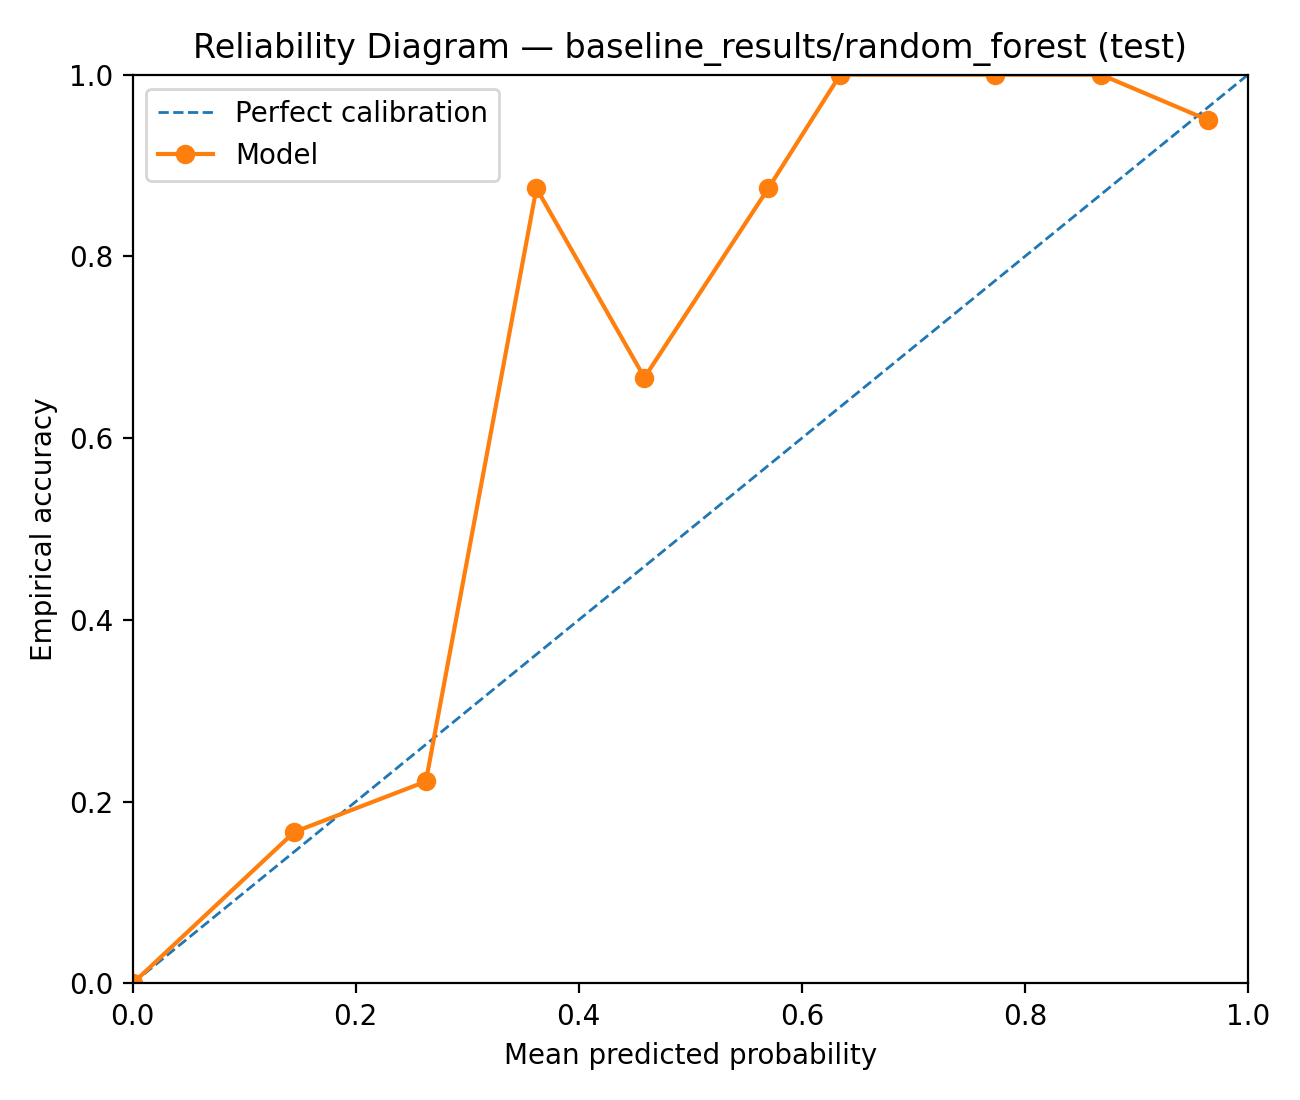
\includegraphics[width=0.95\linewidth]{figures/baseline_results__random_forest_test_reliability.png}
        \caption{Random Forest}
    \end{subfigure}
    \hfill
    \begin{subfigure}[t]{0.32\linewidth}
        \centering
        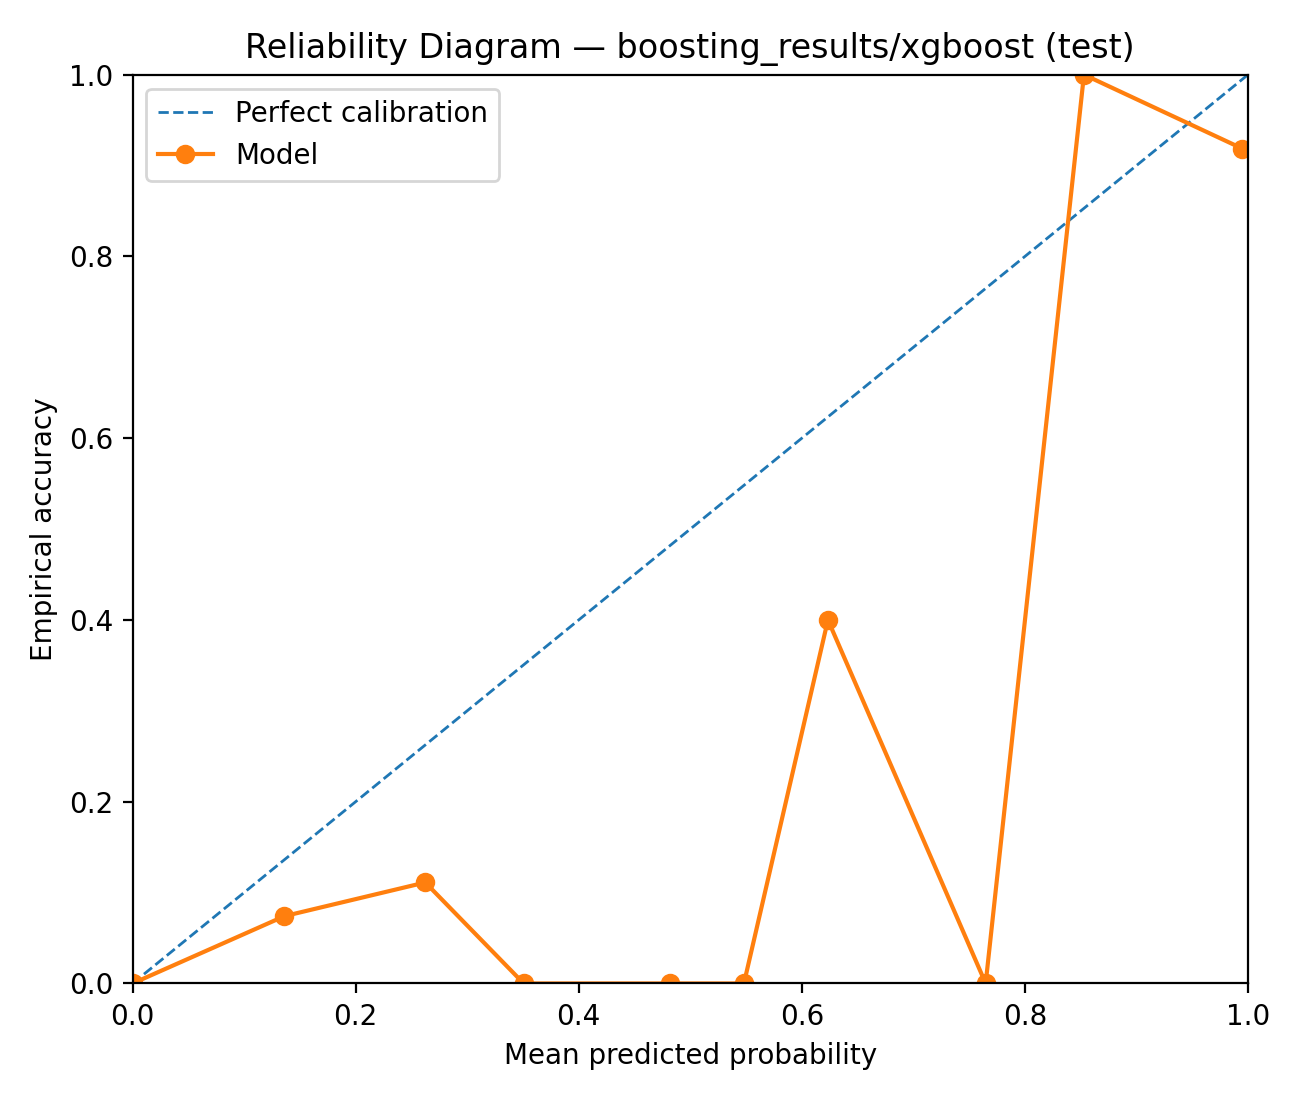
\includegraphics[width=0.95\linewidth]{figures/boosting_results__xgboost_test_reliability.png}
        \caption{XGBoost}
    \end{subfigure}
    \hfill
    \begin{subfigure}[t]{0.32\linewidth}
        \centering
        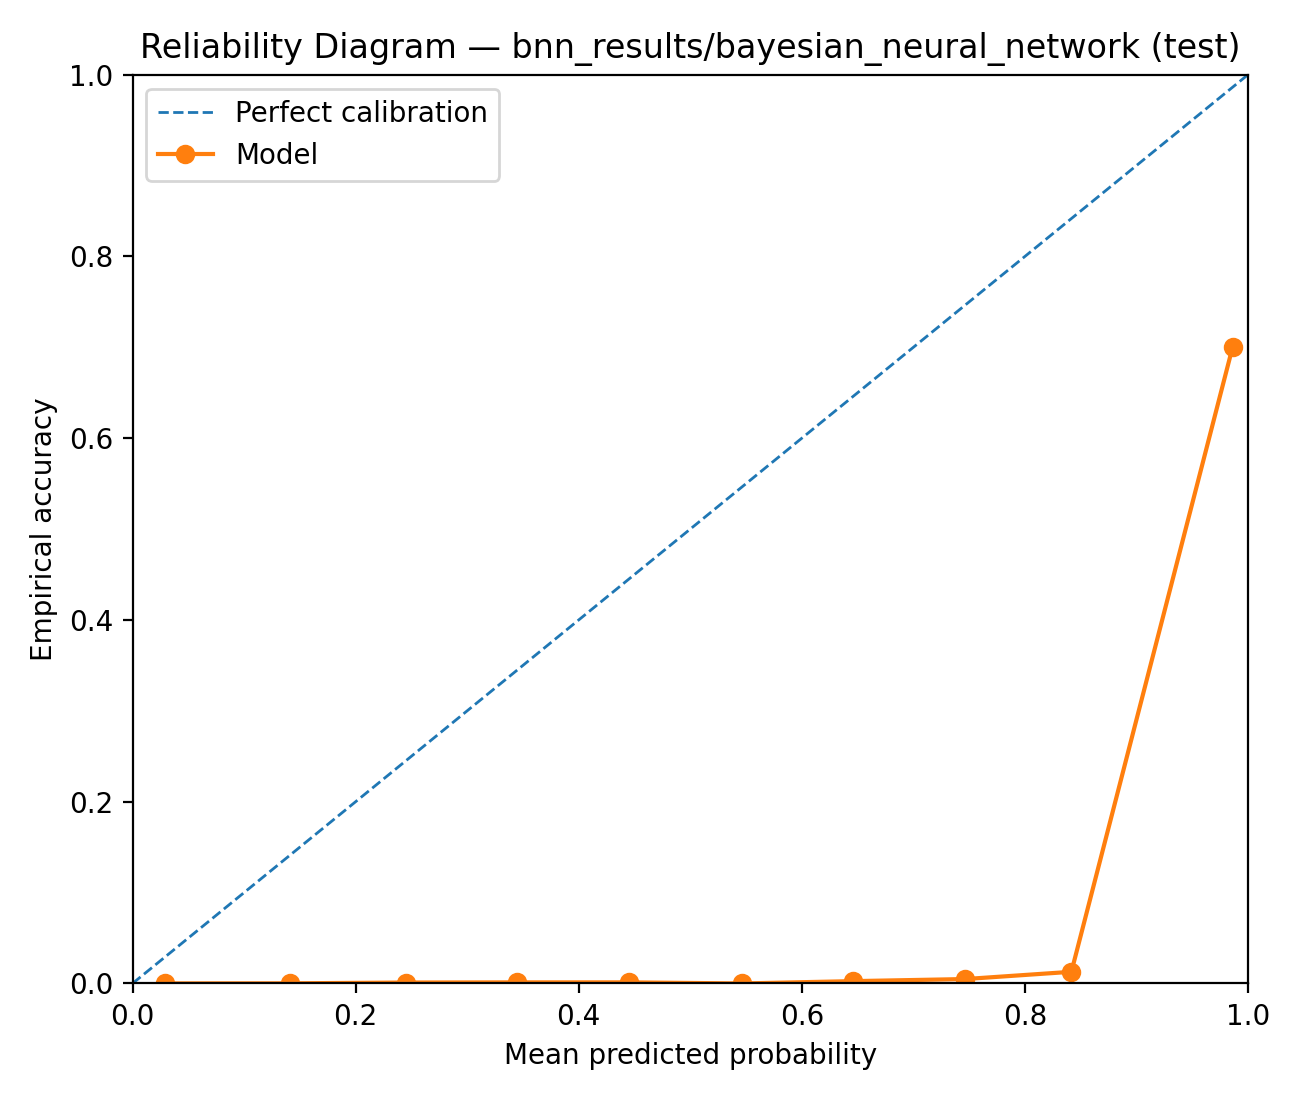
\includegraphics[width=0.95\linewidth]{figures/bnn_results__bayesian_neural_network_test_reliability.png}
        \caption{BNN}
    \end{subfigure}
    \caption{Diagramas de fiabilidad en test.}
    \label{fig:reliability}
\end{figure}

La Tabla~\ref{tab:decision_table} resume la transición desde probabilidad e incertidumbre hacia decisiones accionables. \textsc{Accept} concentra transacciones de riesgo muy bajo; \textsc{Block} recoge una fracción mínima de operaciones, pero con una tasa de fraude extraordinariamente alta; y \textsc{Review} absorbe la región ambigua donde automatizar resultaría más arriesgado.

\begin{table}[!htbp]
    \centering
    \small
    \caption{Resumen de decisiones del BNN en test.}
    \label{tab:decision_table}
    \begin{tabular}{lrrrrr}
        \toprule
        Decisión        & Conteo & Cobertura (\%) & Fraude (\%) & Prob. media (\%) & Incertidumbre media (\%) \\
        \midrule
        \textsc{Accept} & 15424  & 27.1           & 0.006       & 0.6              & 5.4                      \\
        \textsc{Review} & 41451  & 72.8           & 0.060       & 11.2             & 23.5                     \\
        \textsc{Block}  & 87     & 0.15           & 82.8        & 99.9             & 1.8                      \\
        \bottomrule
    \end{tabular}
\end{table}

Este resultado es central para el caso de uso. Más que producir una etiqueta, el sistema redistribuye el espacio de decisiones en tres niveles de intervención. El bucket \textsc{Block} es especialmente informativo: aunque es muy pequeño, concentra una proporción altísima de fraude y lo hace con incertidumbre media baja, lo que encaja con la idea de bloquear únicamente cuando la predicción es extrema y estable. \textsc{Accept}, por el contrario, recoge una parte importante del volumen con riesgo residual muy reducido. La mayor carga operativa recae sobre \textsc{Review}, que actúa como mecanismo de prudencia: absorbe el grueso de las transacciones donde el riesgo o la inestabilidad posterior desaconsejan una decisión totalmente automática.

La Figura~\ref{fig:gplvm_decision} complementa esta lectura mostrando que dichas decisiones se agrupan en regiones diferenciadas del espacio latente. Aunque no existe una separación perfectamente limpia entre las tres clases de decisión, sí aparecen zonas donde \textsc{Review} domina claramente y otras donde ciertos casos \textsc{Block} quedan más apartados. Esto sugiere que la política operativa no es arbitraria, sino que refleja cierta estructura geométrica del espacio inducido por el GPLVM.

\begin{figure}[H]
    \centering
    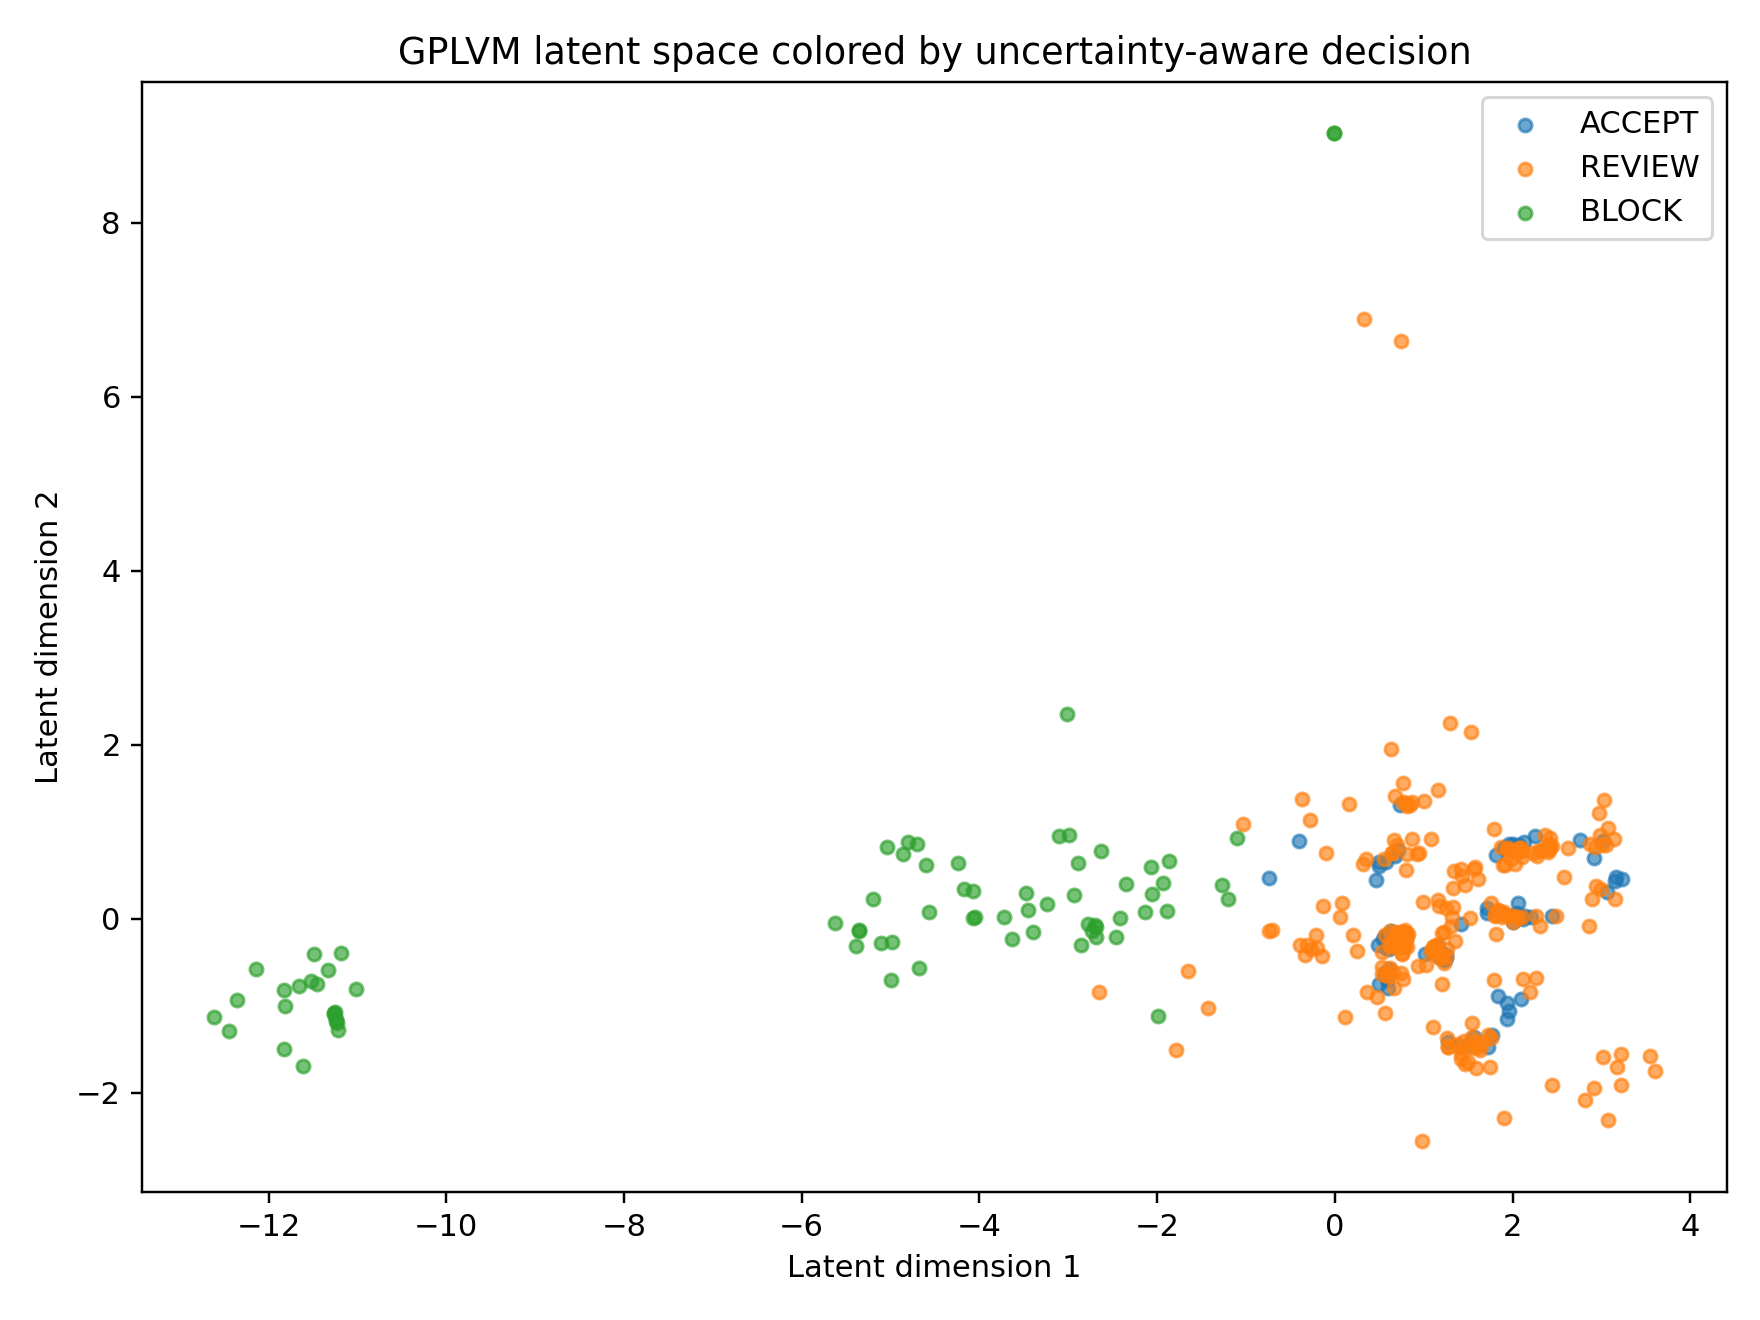
\includegraphics[width=0.60\linewidth]{figures/latent_space_by_decision.png}
    \caption{Espacio latente GPLVM coloreado por decisión.}
    \label{fig:gplvm_decision}
\end{figure}

La Figura~\ref{fig:prob_vs_unc} muestra que la incertidumbre predictiva se concentra en probabilidades intermedias y cae en los extremos cercanos a 0 o 1. Esta estructura es coherente con la interpretación bayesiana del modelo: cuando la posterior predictiva está repartida entre múltiples comportamientos plausibles, la probabilidad media tiende a desplazarse hacia regiones ambiguas y la desviación estándar aumenta.

La forma de arco que aparece en la nube de puntos es especialmente informativa, porque muestra que la incertidumbre no se distribuye al azar. En lugar de eso, aumenta precisamente donde la decisión es menos clara y disminuye cuando la red produce salidas extremas. Esto refuerza la idea de que la incertidumbre puede utilizarse como una señal de segundo nivel para decidir cuánto confiar en la probabilidad predicha.

\begin{figure}[H]
    \centering
    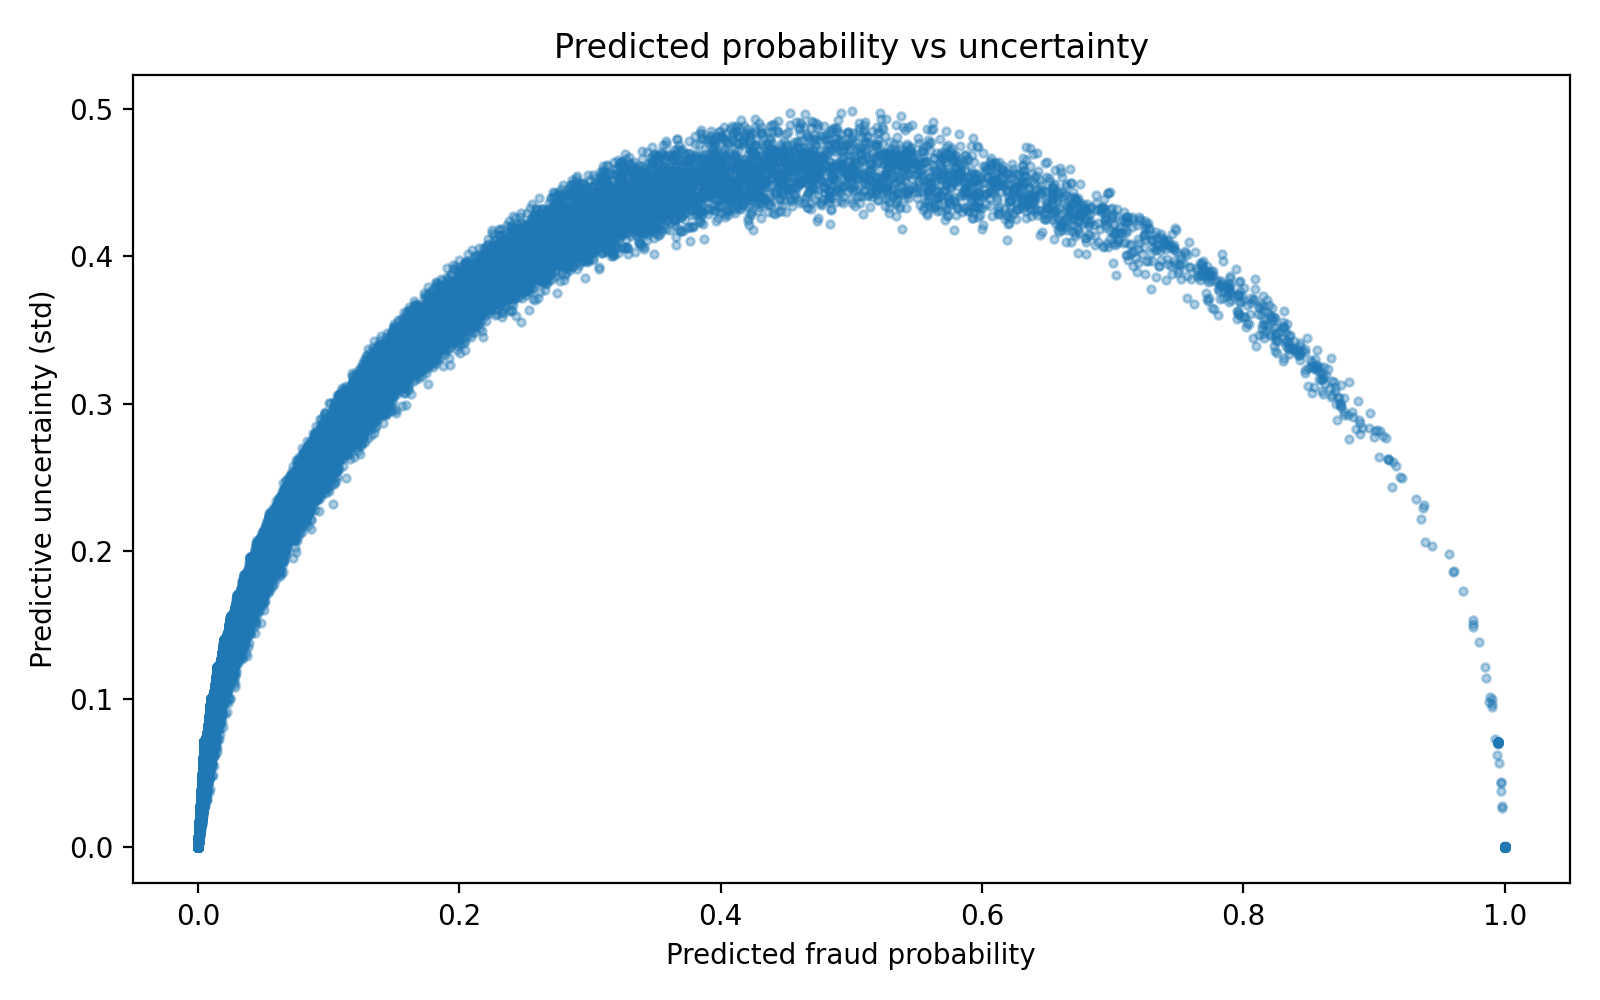
\includegraphics[width=0.60\linewidth]{figures/test_probability_vs_uncertainty.png}
    \caption{Probabilidad predicha frente a incertidumbre del BNN.}
    \label{fig:prob_vs_unc}
\end{figure}

Esta lectura se refuerza con la Figura~\ref{fig:unc_by_confusion}, que añade una observación operativamente relevante: los errores más problemáticos tienden a concentrarse en niveles más altos de incertidumbre.

En particular, los falsos negativos aparecen desplazados hacia valores más altos que los verdaderos positivos, lo cual es importante porque el falso negativo es precisamente el error más costoso en este contexto. La figura no implica que la incertidumbre separe perfectamente aciertos y errores, pero sí sugiere que los casos más delicados se concentran en regiones donde la posterior predictiva es menos estable. Desde el punto de vista operativo, esto refuerza la conveniencia de derivar esos casos hacia revisión en lugar de automatizarlos.

\begin{figure}[H]
    \centering
    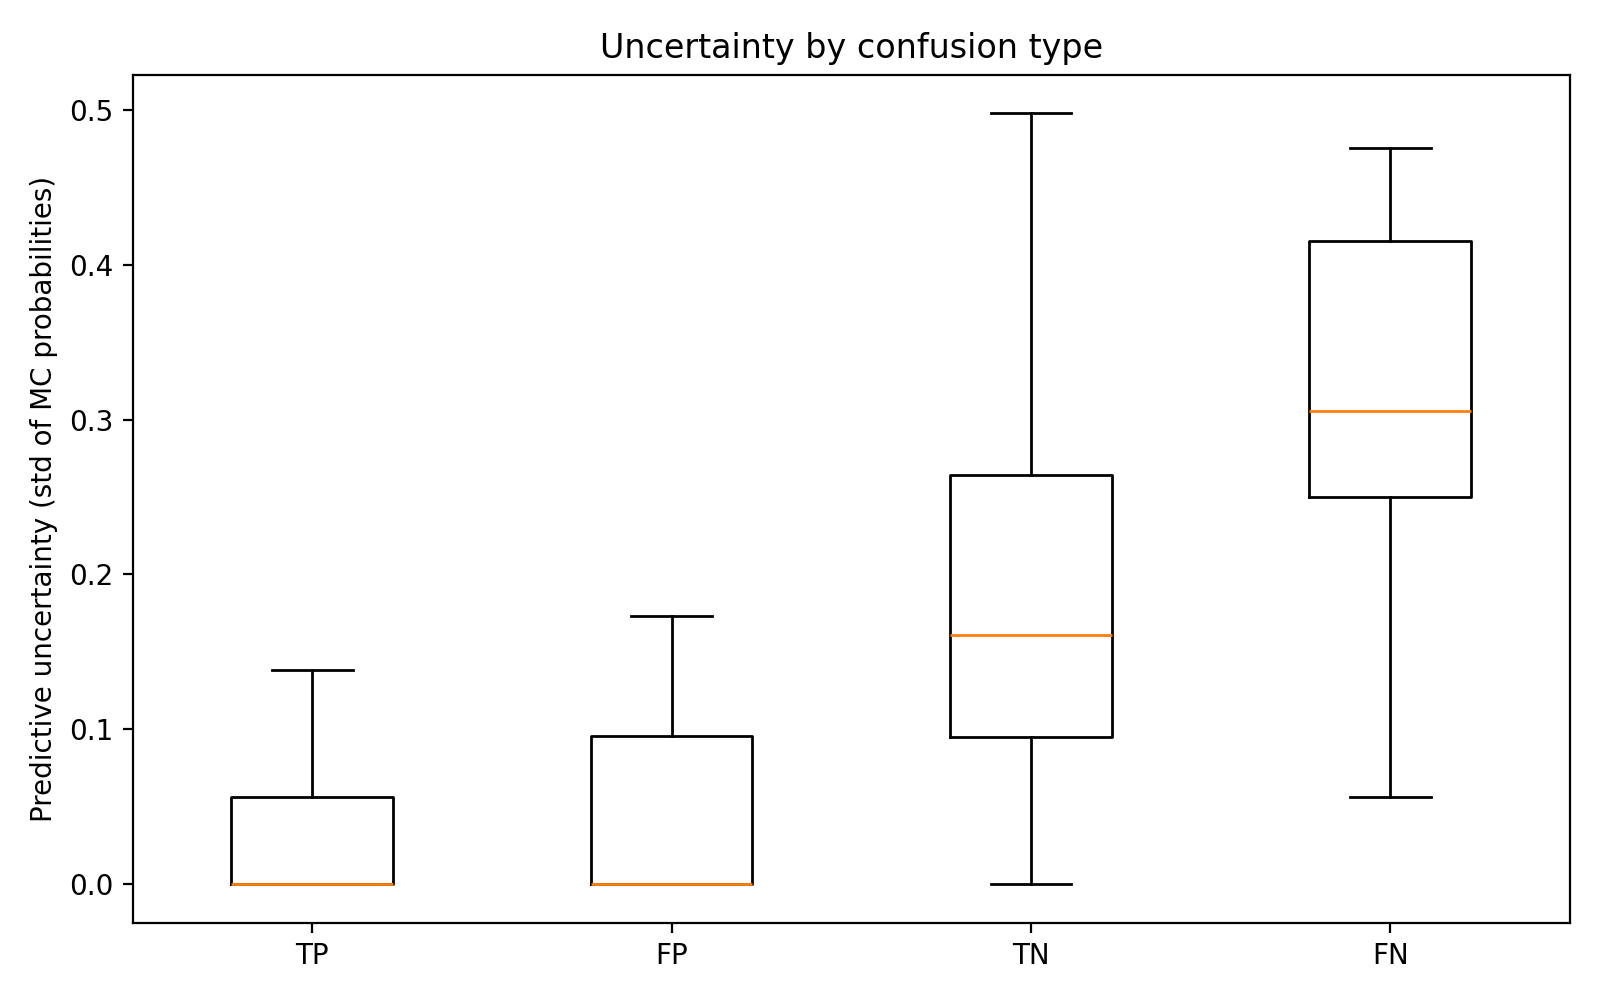
\includegraphics[width=0.60\linewidth]{figures/test_uncertainty_by_confusion_type.png}
    \caption{Incertidumbre por tipo de confusión.}
    \label{fig:unc_by_confusion}
\end{figure}

La Figura~\ref{fig:coverage_risk} formaliza esta idea mediante el análisis riesgo-cobertura. A medida que el sistema restringe la automatización al subconjunto menos incierto, el riesgo empírico disminuye. En consecuencia, la incertidumbre no actúa solo como descriptor estadístico, sino como variable de control para modular la agresividad de la decisión automática.

La caída brusca del riesgo al abandonar las regiones más inciertas sugiere que la señal de incertidumbre efectivamente ordena los ejemplos según su fiabilidad relativa. Aunque la escala del riesgo está condicionada por el fuerte desbalance del problema, la tendencia global es clara: automatizar menos y mejor permite reducir errores sobre el subconjunto retenido. Esta figura, por tanto, no solo respalda la intuición cualitativa de las figuras anteriores, sino que ofrece una justificación cuantitativa de la abstención selectiva.

\begin{figure}[H]
    \centering
    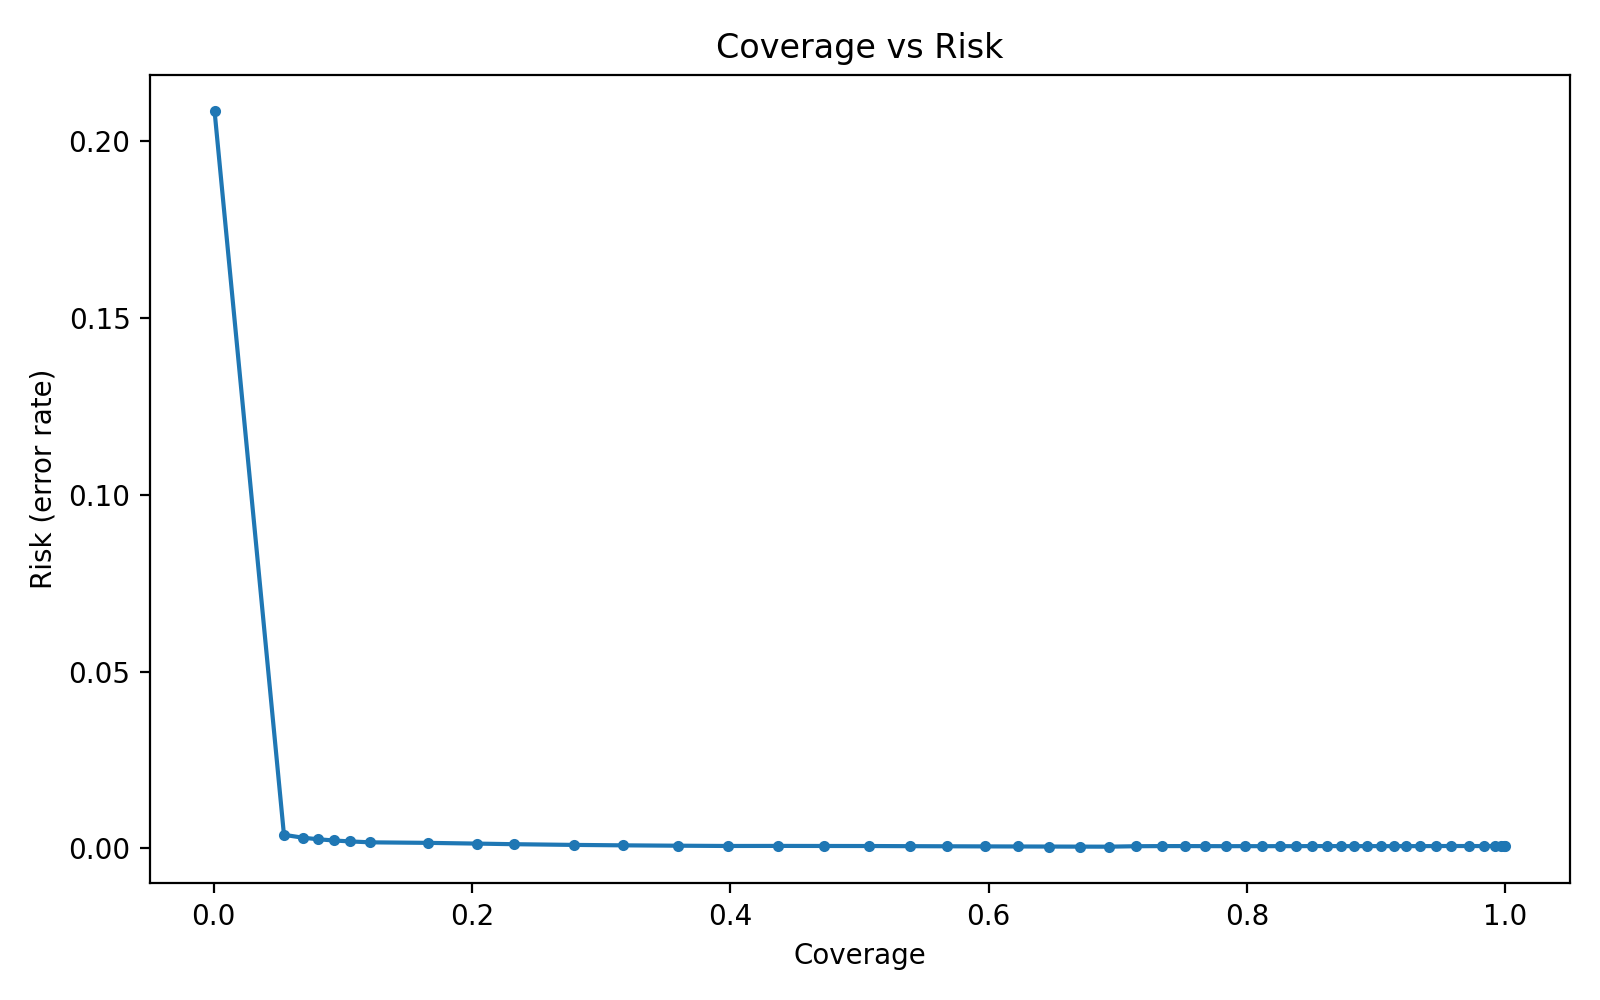
\includegraphics[width=0.60\linewidth]{figures/test_coverage_vs_risk.png}
    \caption{Curva cobertura-riesgo del BNN.}
    \label{fig:coverage_risk}
\end{figure}

Esta parte es una de las evidencias más fuertes del valor práctico del enfoque. Si una señal de incertidumbre es útil, debería permitir mejorar la calidad de las decisiones reteniendo únicamente los casos más fiables; y precisamente eso es lo que sugiere la curva cobertura-riesgo. La lectura operativa es directa: cuanto más restrictivo es el sistema con la automatización, menor es el riesgo asumido sobre el subconjunto automatizado. Por tanto, la incertidumbre puede interpretarse como una herramienta para regular de forma continua el compromiso entre volumen automatizado y seguridad.

Además, el hecho de que la incertidumbre aumente justamente en regiones ambiguas y en tipos de error problemáticos apoya la coherencia interna del enfoque. No se trata solo de que el modelo produzca una desviación estándar numérica, sino de que esa magnitud se alinea con casos donde intuitivamente esperaríamos menor fiabilidad. Esto refuerza la idea de que la BNN añade valor no por superar a los baselines en clasificación, sino por hacer visible qué parte del espacio de decisión debería tratarse con mayor cautela.

\FloatBarrier

La Tabla~\ref{tab:efficiency} resume el coste computacional de los modelos en inferencia. El resultado importante no es únicamente que la BNN sea más lenta, sino por qué lo es: su estimación predictiva requiere muestreo Monte Carlo repetido, lo que eleva significativamente la latencia por muestra.

\begin{table}[!htbp]
    \centering
    \small
    \caption{Eficiencia de inferencia y entrenamiento.}
    \label{tab:efficiency}
    \begin{tabular}{lrrrrr}
        \toprule
        Modelo              & Tamaño (MB) & Carga (s) & Inferencia total (s) & Latencia ($\mu$s/muestra) & Entrenamiento \\
        \midrule
        Logistic Regression & 0.004       & 0.001     & 0.041                & 0.7                       & 1.3 s         \\
        XGBoost             & 0.586       & 0.080     & 0.073                & 1.3                       & 3.4 s         \\
        Random Forest       & 7.508       & 0.235     & 0.180                & 3.2                       & 33.6 s        \\
        BNN (+ prep.)       & 0.323       & 0.020     & 17.689               & 310.5                     & 924 s         \\
        \bottomrule
    \end{tabular}
\end{table}

En otras palabras, el enriquecimiento probabilístico tiene un coste explícito. El uso de una BNN en este contexto solo se justifica si la mejora en control del riesgo compensa la penalización computacional. El sistema incluye además un \emph{frontend} funcional en Streamlit para \emph{batch scoring}, exploración de casos y \emph{dashboard}, así como un \texttt{Dockerfile} para despliegue reproducible. También se implementa una capa de monitorización \emph{snapshot-style} que resume distribución de decisiones, incertidumbre y señales agregadas de riesgo. No se trata de una monitorización online en producción, sino de una primera aproximación reproducible a evaluación post-despliegue.

\paragraph{Consistencia de artefactos.}
Todos los umbrales, métricas y reglas de decisión reportados en este trabajo se derivan directamente de los artefactos experimentales validados, sin ajuste \emph{post hoc}.

\FloatBarrier
\section{Limitaciones y conclusión}

Este trabajo presenta varias limitaciones importantes. Primero, la BNN no supera a los mejores modelos deterministas en ranking predictivo ni en calibración sobre este dataset tabular. Segundo, la incertidumbre usada por el sistema es una dispersión Monte Carlo de la posterior predictiva aproximada, no una descomposición formal entre incertidumbre aleatoria y epistémica. Tercero, la monitorización es offline y de tipo \emph{snapshot}, no un sistema online de producción. Cuarto, los tiempos de entrenamiento no fueron medidos sistemáticamente y por tanto se reportan como \texttt{UNSPECIFIED} para no introducir estimaciones no verificables.

Aun así, la comparación entre modelos probabilísticos y deterministas en fraude debe formularse en dos planos distintos. En el plano predictivo, XGBoost y Random Forest son superiores a la BNN en las métricas más relevantes de discriminación y, en particular, los modelos de árbol presentan una calibración notablemente mejor. En ese sentido, este trabajo no proporciona evidencia de que una BNN sea el mejor clasificador tabular para este dataset.

Sin embargo, en el plano decisional la conclusión es distinta. La BNN permite construir una política de abstención explícita, identificar una fracción pequeña pero muy concentrada de operaciones de alto riesgo y desplazar a revisión humana los casos donde la automatización sería más frágil. La combinación de la Tabla~\ref{tab:decision_table} y la Figura~\ref{fig:coverage_risk} sugiere precisamente eso: la incertidumbre estimada por el modelo no es solo un subproducto estadístico, sino una variable útil para gestionar el riesgo operativo.

La comparación final, por tanto, no es simplemente entre ``mejor'' y ``peor'' modelo. Si el objetivo fuese únicamente maximizar rendimiento predictivo offline, los modelos de árbol serían la opción natural. Si, en cambio, el objetivo incluye controlar mejor cuándo automatizar, cuándo derivar y cuándo aceptar el coste de una revisión humana, entonces la BNN ofrece una ventaja cualitativamente distinta. Ese es el trade-off central del trabajo: renunciar a parte del rendimiento puro a cambio de una señal explícita de incertidumbre que permite tomar decisiones más prudentes y más adaptadas al coste del error.

La conclusión principal no es que el modelo bayesiano sea globalmente mejor, sino que permite transformar una predicción binaria en una política de decisión más segura. En aplicaciones sensibles al riesgo, esa capacidad puede justificar su uso incluso cuando no domina en PR-AUC o NLL.

\begin{thebibliography}{99}

    \bibitem[Blundell et~al.(2015)Blundell, Cornebise, Kavukcuoglu, and Wierstra]{blundell2015}
    Charles Blundell, Julien Cornebise, Koray Kavukcuoglu, and Daan Wierstra.
    \newblock Weight uncertainty in neural networks.
    \newblock In \emph{Proceedings of the 32nd International Conference on Machine Learning}, 2015.

    \bibitem[Dal~Pozzolo et~al.(2015)Dal~Pozzolo, Caelen, Johnson, and Bontempi]{dalpozzolo2015}
    Andrea Dal~Pozzolo, Olivier Caelen, Reid A. Johnson, and Gianluca Bontempi.
    \newblock Calibrating probability with undersampling for unbalanced classification.
    \newblock In \emph{IEEE Symposium Series on Computational Intelligence}, 2015.

    \bibitem[El-Yaniv and Wiener(2010)]{elyaniv2010}
    Ran El-Yaniv and Yair Wiener.
    \newblock On the foundations of noise-free selective classification.
    \newblock \emph{Journal of Machine Learning Research}, 11:1605--1641, 2010.

    \bibitem[Gal and Ghahramani(2016)]{gal2016}
    Yarin Gal and Zoubin Ghahramani.
    \newblock Dropout as a Bayesian approximation: representing model uncertainty in deep learning.
    \newblock In \emph{Proceedings of the 33rd International Conference on Machine Learning}, 2016.

    \bibitem[Gneiting and Raftery(2007)]{gneiting2007}
    Tilmann Gneiting and Adrian E. Raftery.
    \newblock Strictly proper scoring rules, prediction, and estimation.
    \newblock \emph{Journal of the American Statistical Association}, 102(477):359--378, 2007.

    \bibitem[Guo et~al.(2017)Guo, Pleiss, Sun, and Weinberger]{guo2017}
    Chuan Guo, Geoff Pleiss, Yu Sun, and Kilian Q. Weinberger.
    \newblock On calibration of modern neural networks.
    \newblock In \emph{Proceedings of the 34th International Conference on Machine Learning}, 2017.

    \bibitem[Kaggle(2016)]{kagglecreditcard}
    Kaggle.
    \newblock Credit Card Fraud Detection.
    \newblock \url{https://www.kaggle.com/datasets/mlg-ulb/creditcardfraud}, consultado el 17 de abril de 2026.

    \bibitem[Kingma and Welling(2014)]{kingma2014}
    Diederik P. Kingma and Max Welling.
    \newblock Auto-encoding variational Bayes.
    \newblock In \emph{International Conference on Learning Representations}, 2014.

    \bibitem[Lawrence(2005)]{lawrence2005}
    Neil D. Lawrence.
    \newblock Probabilistic non-linear principal component analysis with Gaussian process latent variable models.
    \newblock \emph{Journal of Machine Learning Research}, 6:1783--1816, 2005.

    \bibitem[Niculescu-Mizil and Caruana(2005)]{niculescu2005}
    Alexandru Niculescu-Mizil and Rich Caruana.
    \newblock Predicting good probabilities with supervised learning.
    \newblock In \emph{Proceedings of the 22nd International Conference on Machine Learning}, 2005.

    \bibitem[Pyro Development Team(2026a)]{pyroautoguide}
    Pyro Development Team.
    \newblock Automatic guide generation: \texttt{AutoDiagonalNormal}.
    \newblock \url{https://docs.pyro.ai/en/stable/infer.autoguide.html}, consultado el 17 de abril de 2026.

    \bibitem[Pyro Development Team(2026b)]{pyrosvi}
    Pyro Development Team.
    \newblock Stochastic variational inference in Pyro.
    \newblock \url{https://docs.pyro.ai/en/stable/inference_algos.html}, consultado el 17 de abril de 2026.

    \bibitem[Pyro Development Team(2026c)]{pyropredictive}
    Pyro Development Team.
    \newblock Predictive distribution in Pyro.
    \newblock \url{https://docs.pyro.ai/en/stable/_modules/pyro/infer/predictive.html}, consultado el 17 de abril de 2026.

\end{thebibliography}

\end{document}